%\documentclass[a4paper,10pt]{jarticle}
%\documentclass[]{jarticle}
\documentclass[10pt]{jarticle}

%\usepackage{graphicx}
\usepackage[dvipdfmx]{graphicx}
\usepackage{eclbkbox} %breakbox用
\usepackage{amsmath,amssymb}
\usepackage{verbatim}
\usepackage{moreverb}
\usepackage{ascmac,here,txfonts,txfonts}
\usepackage{listings,jlisting}
\usepackage{color}
\usepackage{fancybox}

%本文領域を広め(空白箇所マージン領域を小さめ)に設定
\lstset{
  breaklines = true,
  language=Python,
  basicstyle=\ttfamily\scriptsize,
  commentstyle={\itshape \color[cmyk]{1,0.4,1,0}},
  classoffset=1,
  keywordstyle={\bfseries \color[cmyk]{0,1,0,0}},
  stringstyle={\ttfamily \color[rgb]{0,0,1}},
  frame=tRBl,
  framesep=5pt,
  showstringspaces=false,
  numbers=left,
  stepnumber=1,
  numberstyle=\tiny,
  tabsize=2,
}

\setlength{\textwidth}{179mm}
\setlength{\textheight}{251mm}
\setlength{\topmargin}{-2cm}
\setlength{\oddsidemargin}{-1cm}
\setlength{\evensidemargin}{-1cm}

\begin{document}

\title{情報工学実験IIレポート(探索アルゴリズム1)}
\author{月曜日&グループ7} %
\date{2014年12月15日}

\maketitle

%\begin{abstract}
% この骨組み(テンプレート)を利用する際には、
% 不要な箇所を削除した上で提出すること。
% 例えばこの要旨やコメント文の殆どは
% 「當間から学生へのコメント」であって、
% 「課題に対するレポート(報告書)」ではない。
% 
% このレポート(ファイル)は、「情報工学実験II・探索アルゴリズムその
% 1\cite{info2-search1}」の実験レポートの骨組みを例示している。
% あくまでも例示であって、全てをこの通りに従う必要はないが、
% 指示された項目を含めた上で、
% 報告書として他者が読みやすいレポートとなるよう考慮すること。
%\end{abstract}

\section*{グループメンバ}
%(補足:レベル毎に \underline{全員が協力して実施} した上で、レベル毎にレポートをまとめる担当者を決め、全体を一つのレポートとして整理すること。分担方法も自由である。)
\begin{itemize}
 \item 135711F 屋比久祐樹: 担当Level1.1, 2.2
 \item 135713B 天願寛之: 担当Level2.1
 \item 135717E 岡田和也: 担当Level3.1, 4.1
 \item 135761B 大城海斗: 担当Level1.2,2.3
\end{itemize}

\section*{提出したレポート一式について}
レポート一式は
``\verb|shell:/net/home/teacher/tnal/2014-search1-mon/group7/|''
にアップロードした。
提出したファイルのディレクトリ構成は以下の通りである。

\vspace{+0.5cm}
\begin{breakbox}
\begin{verbatim}
./           #レポート等
./figs/      #図表や実験に必要なプログラムなど.

\end{verbatim}
\end{breakbox}

\newpage

\section{Leve l1: 探索とは}
\subsection{Level1.1: コンピュータと人間の違いを述べよ}
\subsubsection{課題説明}
コンピュータが人間より得意とするモノ、その反対に人間より不得手のモノ、両者について2つ以上の視点(立場や観点など)を示し、考察する。\\
\\
・コンピュータはパターン化されたものを決まった動作を繰り返す。\\
・コンピュータは大量の情報を取り扱いや特定のパターンに基づいてまとめたりする。\\
\\
・コンピュータの不得意なことは、感情移入判断することが出来ない、決まったことしか出来ない。\\
・コンピュータと違いは、パターン化されていないことも出来る
\subsubsection{考察}
\begin{itemize}
 \item 視点1: \\
コンピュータは、パターン化されたことが得意\\
 \item 視点2: \\
人間は、パターン化されないことでも出来る\\
\end{itemize}


\subsection{Leve1.2: 評価方法(目的関数の設計指針や方法)について}
\subsubsection{課題説明}
Amazonにおける書籍検索時に「ファンタジー作品で泣ける作品」を探し出すため
のアイテム集合$x$と目的関数$f(x)$について検討した。

% アイテム集合x: 目的関数に入力されるxは何か?
% 目的関数f(x): 入力されたxをどのように評価したら良いか?
% (オプション) 上記で設計した目的関数の欠点があれば例示と共に解説せよ。

\subsubsection{アイテム集合$x$について}
%私達のグループはhogeをfugaすることについて検討を進めた。すなわち云々

我々のグループでは,ファンタジー作品のレビューに書いてあるワードをアイテム集合$x$とすることを考えた.
次のようなレビューを例にとると,レビューに書いてあるすべての単語がアイテム集合$x$になる.
\begin{quote}
いやぁ、おもしろい。
異世界ファンタジーと言うのは、最初の数ページでこれはちょっと、と思う場合と、そこ
で引き込まれてあっという間と言う場合の二種類がある気がするけど、本書はもちろん後
者の方。
ありえなぁいと叫ぶだけのような、そんな浅いファンタジーではなく、とてもとても重厚
な、しっかり細部も練り込まれた、実に味わい深い作品でした。
\end{quote}

\subsubsection{目的関数について}
目的関数$f(x)$はすべてのアイテム集合$x$(レビュー内容の単語)に対して
重み付けをし,それを足し合わせた合計を返す関数とする.
先ほどのレビューを例にとると,「おもしろい」や「重厚な」,「味わい深い」などの作品を高く評価する単語に対しては
他のワードより大きな値を付加する.
そして探索目的は値が最大になるような$f(x)$である(図\ref{fig:level1-2}参照).

% (補足:PDF図を挿入する例)

\begin{figure}[h]
	\begin{center}
		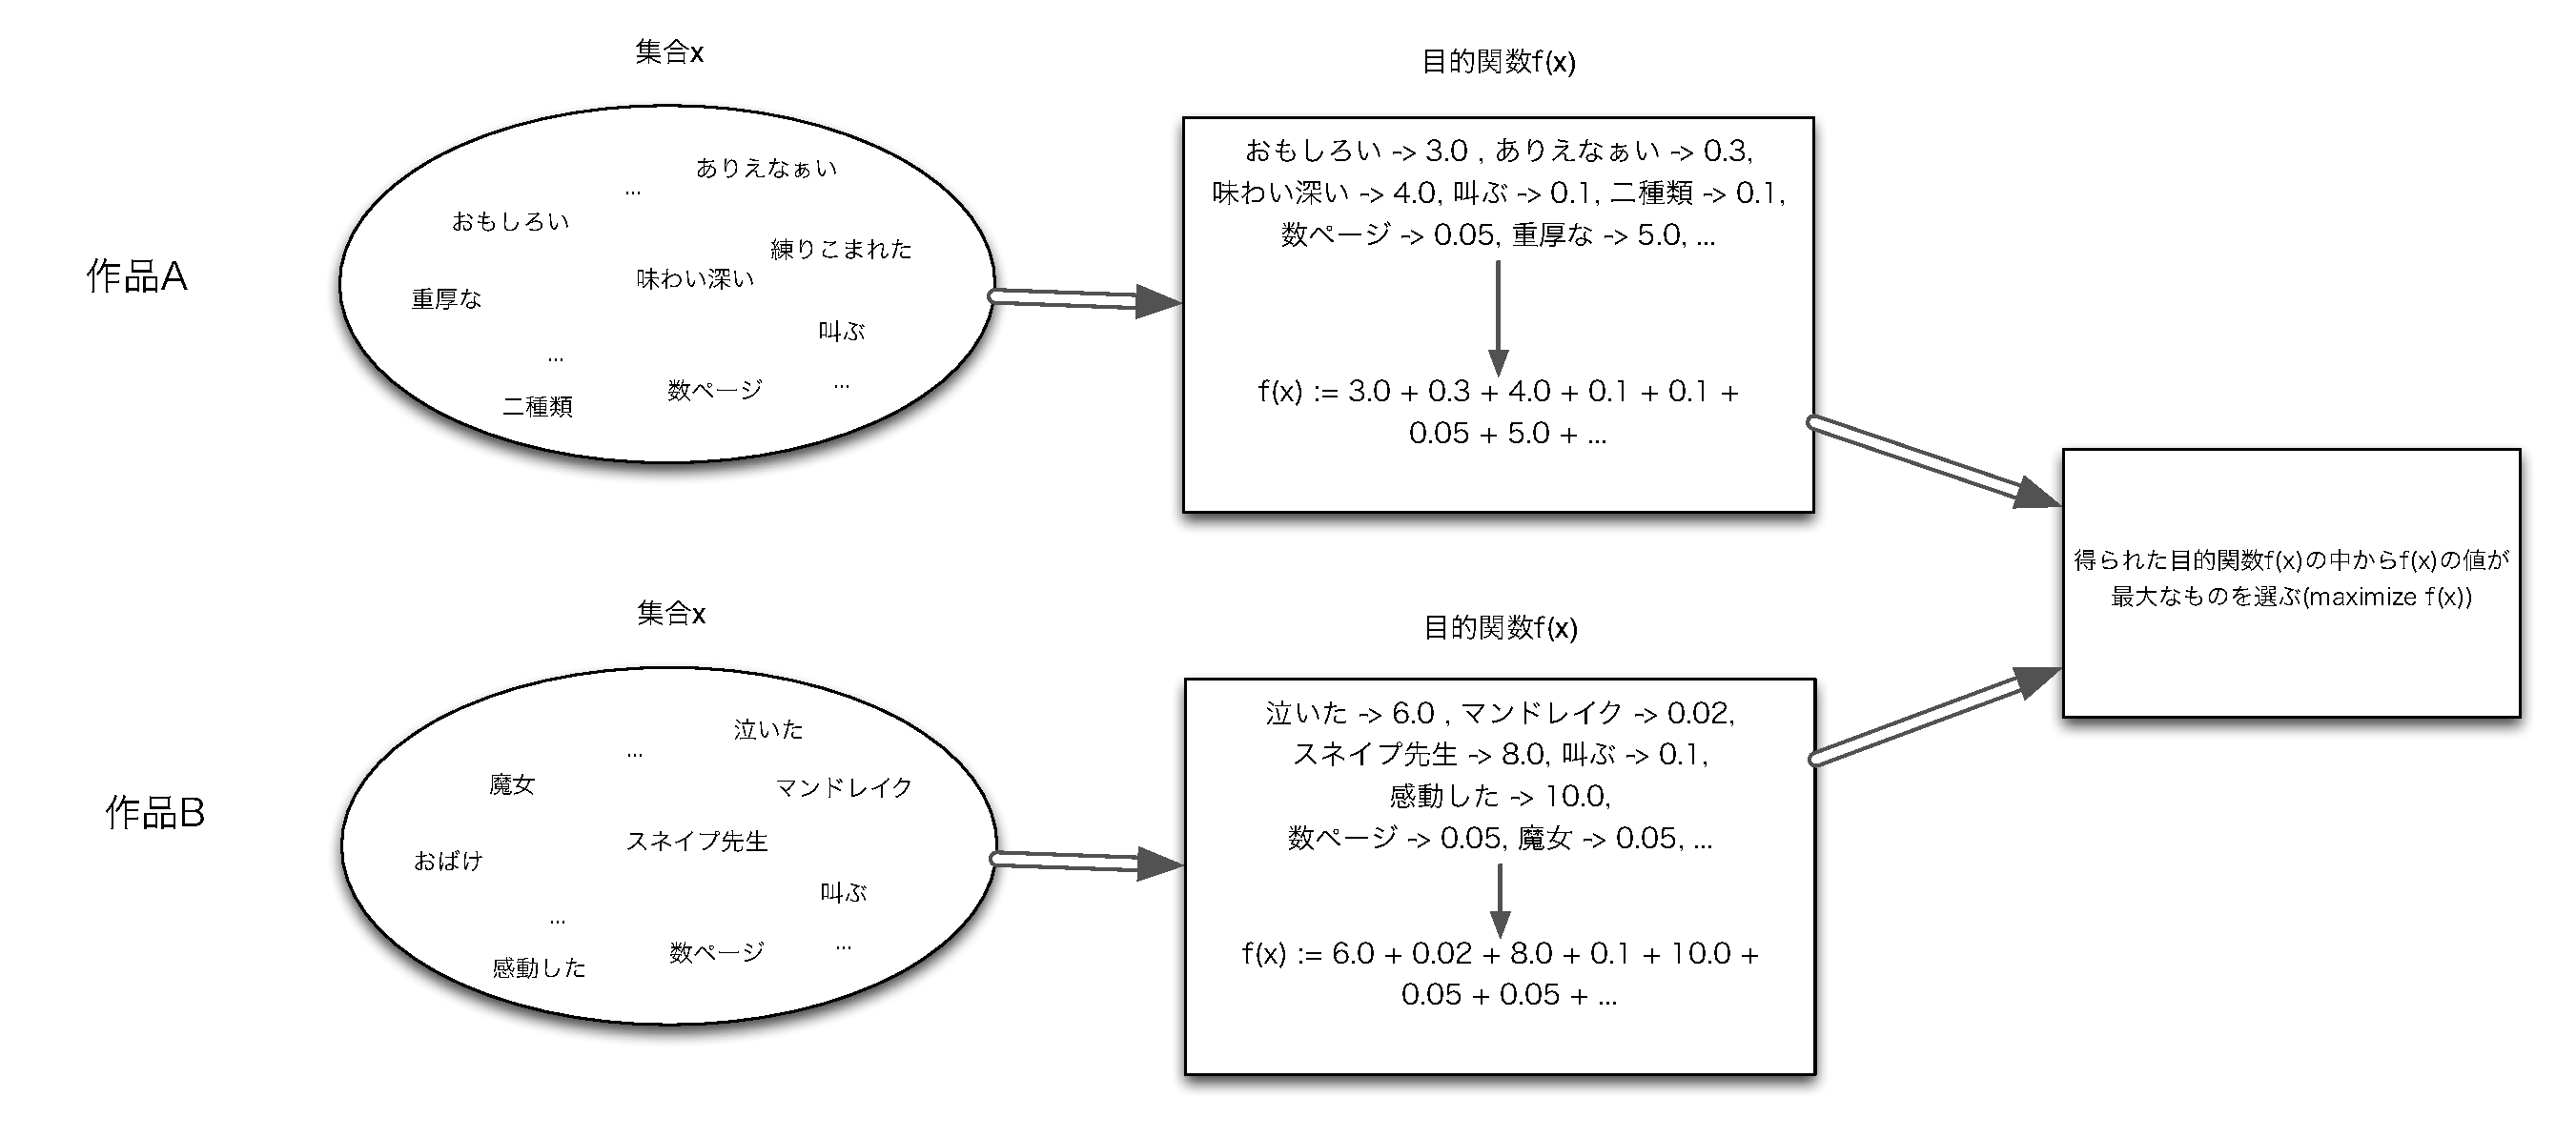
\includegraphics[scale=0.35]{./figs/level1-2.eps}
	\end{center}
	\caption{泣ける作品を探し出すまでの流れ}
	\label{fig:level1-2}
\end{figure}

\subsubsection{目的関数の欠点}
この目的関数の設計上の問題点は
あらかじめワードとワードに対応する重みの値を定義しておく必要があるということである.



\newpage

\section{Level 2: 最急降下法による最適化}
\subsection{課題説明}
3種類の連続関数$y=x^2$、$z=x^2+y^2$、$y=-x \times sin(x)$について、
最急降下法の適用を通して探索挙動を観察した。
以下ではまず共通部分である最急降下法の探索手続きについて、
フローチャートを用いて解説する。
その後、3種類の関数毎にプログラムの変更箇所、
観察意図観察方法、観察結果、考察について説明する。
\subsection{Level 2共通部分}

\subsubsection{探索の手続きとフローチャート(共通部分)}
\begin{figure}[htbp]
  \begin{center}
    \includegraphics[clip,width=7.0cm]{./figs/tonal1.pdf}
    \caption{探索手続きのフローチャート}
 \end{center}
\end{figure}
 %共通部分の結果及び考察
\subsection{Level2.1: $y=x^2$}
\subsubsection{プログラムソース}
\lstinputlisting[caption=変更された関数f(x\,y),label=ラベル]{./figs/f2-1.txt}
\lstinputlisting[caption=変更されたf(x\,y)の微分値,label=ラベル]{./figs/x2-1.txt}
\subsubsection{観察意図と観察方法(実験計画)}
変更したプログラムに対して、シード値を1、α値を0.1として実行する。run\_ave.shファイルの実行結果により、シード値が及ぼす挙動についてみれるはずなので、その結果をもとにシード値の考察を行う。次にα値により探索点の推移距離が変わるので、シード値を固定したままα値をより大きく、または小さくした値に変更して実験を行うことでα値が探索挙動に及ぼす影響を考察する。この時、関数に対して谷が1つなのでxの解やα値が1つに定まるはずなのでそれを意識する。
\subsubsection{実行結果}
\lstinputlisting[caption=\.\/steepest\_decent 1の実行結果,label=ラベル]{./figs/hoge2-1.txt}
シード値を1、α値を0.1に設定して実行した結果、xの値が-7.3692442371から始まり、step63でf(x)の値が0、
探索点がほとんど動かなくなった為step75で終了した。\\
./run\_ave.shを用いてシード値を千刻み10パターン(1000〜10000)で実行し平均試行回数を計測した。1000〜10000までそれぞれの試行回数は順に64、75、69、74、71、73、73、72、74、70であり、平均試行回数は71.5stepであった。
\newline
\begin{figure}[htbp]
  \begin{center}
    \begin{tabular}{c}

      % 1
      \begin{minipage}{0.5\hsize}
        \begin{center}
          \includegraphics[clip, width=7cm]{./figs/sim2-1_step-1.eps}
          \hspace{1.6cm} 図1 stepあたりの目的関数推移線グラフ
        \end{center}
      \end{minipage}

      % 2
      \begin{minipage}{0.5\hsize}
        \begin{center}
          \includegraphics[clip, width=7cm]{./figs/sim2-1-1.eps}
          \hspace{1.6cm} 図2 探索点が関数上をどのように推移したかを示すグラフ
        \end{center}
      \end{minipage}

    \end{tabular}
  \end{center}
\end{figure}
\newline
図1と図2はシード値1、αを0.1に設定して実行された最急降下法アルゴリズムにおける点のstepあたりの移線グラフと関数上での推移グラフである。
\subsubsection{考察}
シード値は探索点の初期値の設定に用いるものである。実験結果よりシード値による高さの決定はランダムであるが、α値を固定した場合は、決定した高さがより低いほうがstep数は少ない事が分かった。さらにコマンド「tail -1 .archive-*」を実行した結果、高さと得られる解の質は関係がないと考えられた。\\
α値に関しての考察を得るためシード値1、α値0.1における実験に対してα値を変更した2つの実験を行う。シード値を固定したままα値を0.3、0.007に変更する。シード値は固定であるため開始地点は同じになる。
\lstinputlisting[caption=α値0.3、0.007に置ける\.\/steepest\_decent 1の実行結果,label=ラベル]{./figs/huga2-1.txt}
\begin{figure}[htbp]
  \begin{center}
    \begin{tabular}{c}

      % 1
      \begin{minipage}{0.5\hsize}
        \begin{center}
          \includegraphics[clip, width=7cm]{./figs/sim2-1-0_3.eps}
          \hspace{1.6cm} 図3 探索点の関数上での推移を示すグラフ(α値0.3)
        \end{center}
      \end{minipage}

      % 2
      \begin{minipage}{0.5\hsize}
        \begin{center}
          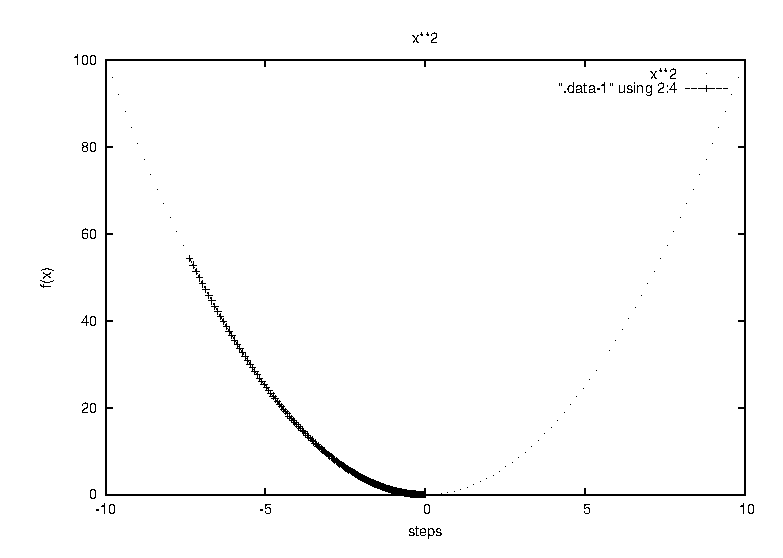
\includegraphics[clip, width=7cm]{./figs/sim2-1-0_007.eps}
          \hspace{1.6cm} 図4 探索点の関数上での推移を示すグラフ(α値0.007)
        \end{center}
      \end{minipage}

    \end{tabular}
  \end{center}
\end{figure}
α値を変更する事で推移距離が変わる。α値を0.3にすると推移距離が長くなり、小さくすると短くなる。\\
α値を0.3にすると、α値0.007、0.1に比べ、step21で探索が済んでいるため効率性がよく、得られる解の質に関しても、誤差が小さくなっていることが実行結果より判断出来る。\\
α値を小さくすると誤差がより大きくなってしまったことに関しては、小さいと探索点から動いていないと判断されてしまい、探索を打ち切られてしまうからと考えられる。\\
これらの実行結果より、3つのα値の内0.3付近がより、探索における有用性が見いだせる。今回の場合、最小値の値が0であり、傾きの値が0となる点であることが自明である。よって移動先の算出は式から見いだせ、その値はα値が0.5のときである。つまりα値が0.5の時step2で最適値を見つけ出す事ができ、解の質においても誤差はない。今回の実験で、0.3付近でより有用性が見いだせたのは、より0.5に近かったからと判断できる。


\subsection{Level2.2: $z=x^2 + y^2$ について}
\subsubsection{プログラムソース(変更部分)}
ソース変更:\\
/** 以下の式を編集して完成させよ(1) **/\\
 $ z = x*x + y*y$;\\
/** 以下の式を編集して完成させよ(2-1) **/\\
$z\_dx = 2*x$;\\
/** 以下の式を編集して完成させよ(2-2) **/\\
$z\_dy = 2*y$;\\
この三カ所である。\\
\subsubsection{観察意図と観察方法}
alphaの数字を変えてみて、どのようになるのかを確認して行く。./trans\_xy\_vs\_func.sh''x**2+y**2''1を用いて、グラフの図を作成しどのようになっているのかを確認した。\\
\subsubsection{実行結果}
alpha = 0.1の時\\
/Users/e135711/実験2/steepestsearch ./trans\_xy\_vs\_func.sh''x**2+y**2'' 1\\
FINISH 3 step 75 x and y were not updated.\\
\\
alpha =1.0の時\\
/Users/e135711/実験2/steepestsearch ./trans\_xy\_vs\_func.sh ''x**2+y**2'' 1\\
FINISH 1 step 1000 this trial couldn't be search enough under the term\_cond=1000.\\
\\
\subsubsection{考察}
 x軸とy軸から見て“.data-1” using2:3:4を確認すると、alphaの数を変えてみた結果、数字を上げて行くと計算回数が少なくなり、数字を下げると計算回数が多くなった。\\

\subsection{Level2.3: $y=-x*sin(x)$ について}

% 問題意識: 効率良く最適解(目的物)を探し出すにはどうしたら良いだろうか?
% 
% Level2.xでは、解空間が連続値であり、目的関数や制約条件が数式として定義されているという前提で「最適値を効率良く求める」ことについて理解を深めていこう。

% レポートに含める項目
% プログラムソース(スクリプトを含む)。
% レポート内には変更個所のみを記載した上で、ソース全体はアップロード提出すること。
% 
% 観察意図と観察方法(実験計画)。コメント: どうやれば最適性or効率性を検討できるだろうか?
% 実行結果。
% 無駄に全てを示す必要はなく、第三者が読んでも理解できる程度に、必要十分に示すこと。
% 
% 考察。
% 特に「学習係数が探索挙動に及ぼす影響」として「得られた解の質」と「効率性」について考察すること。 (どう検証したら良いだろうか?)
% 
% 必要に応じて適切な図表を作成し、理解しやすい考察となるようにすること。


% 今回は「最適性」と「効率性」という視点で考察できるように実験計画を練ってみてください。
\subsubsection{プログラムソース(変更部分)}
Level2.3ではsteepest\_decent.cのf関数とpd\_x関数を一部以下のように変更した.
\begin{itembox}[c]{f(x,y)関数の変更点}
    {\small
    \begin{verbatim}
    double f(double x, double y) {
        double z;

        /** 以下の式を編集して完成させよ(1) **/
        //z = x;
        z = -x * sin(x);

        return( z );
    }
    \end{verbatim}
}
\end{itembox}

\begin{itembox}[c]{pd\_x(x,y)関数の変更点}
    {\small
    \begin{verbatim}
    double pd_x(double x, double y) {
        double z_dx;

        /** 以下の式を編集して完成させよ(2-1) **/
        //z_dx = 1;
        z_dx = -sin(x) - x*cos(x);

        return( z_dx );
    }
\end{verbatim}
}
\end{itembox}

\subsubsection{観察意図と観察方法(実験計画)}
最急降下法は,$y=x^2$のような「極小値=関数全体の最小値」となる
関数に対しては非常に有効なアルゴリズムである.
しかし,今回の$y=-xsin(x)$のように極小値が複数ある場合は,
探索開始地点から最寄りの極小値に収束しようとする.
これは必ずしも関数の最小値だとは限らない.
そのため,複数の初期値を与えて実行し,それぞれの収束したときの
$y$の値の中から最も小さいものを選択すれば,それが関数の最小値
となるだろうと考えた. \\
 run\_ave.shをベースに試行回数10回分の結果の中から$y$の最小値を
抜き出すスクリプト(ソースコード\ref{alter})を作成した.
また学習係数$\alpha$を変えることにより,どのようにstep数が
変動するかを観察する.

\lstinputlisting[caption=$y$の最小値を求めるプログラム,label=alter]{./figs/alter_run_ave.sh}


\subsubsection{実行結果}
% alter_hogehoge.shとrunなんちゃら,trans_step,trans_x_も
% やる
%
今回試した学習係数$\alpha$は$0.075, 0.2$の2つである.
まず,ソースコード\ref{alter}を実行した結果を示す.

\begin{itembox}[c]{$\alpha=0.075$の時に求まった$-xsin(x)$の最小値}
    {\small
        \begin{verbatim}
        /Users/e135761/search/steep/steepestsearch% ./alter_run_ave.sh
        FINISH 3 step 72 x and y were not updated.
        FINISH 3 step 17 x and y were not updated.
        FINISH 3 step 59 x and y were not updated.
        FINISH 3 step 19 x and y were not updated.
        FINISH 3 step 67 x and y were not updated.
        FINISH 3 step 23 x and y were not updated.
        FINISH 3 step 24 x and y were not updated.
        FINISH 3 step 68 x and y were not updated.
        FINISH 3 step 19 x and y were not updated.
        FINISH 3 step 61 x and y were not updated.
        -7.9167273716
        /Users/e135761/search/steep/steepestsearch%
        \end{verbatim}
    }
\end{itembox}

\begin{itembox}[c]{$\alpha=0.2$の時に求まった$-xsin(x)$の最小値}
    {\small
        \begin{verbatim}
        /Users/e135761/search/steep/steepestsearch% ./alter_run_ave.sh
        FINISH 3 step 24 x and y were not updated.
        FINISH 3 step 36 x and y were not updated.
        FINISH 3 step 19 x and y were not updated.
        FINISH 3 step 35 x and y were not updated.
        FINISH 3 step 22 x and y were not updated.
        FINISH 3 step 38 x and y were not updated.
        FINISH 3 step 36 x and y were not updated.
        FINISH 3 step 22 x and y were not updated.
        FINISH 3 step 34 x and y were not updated.
        FINISH 3 step 20 x and y were not updated.
        -7.9167273716
        /Users/e135761/search/steep/steepestsearch%
        \end{verbatim}
    }
\end{itembox}
特に$\alpha$による最小値の違いは見られなかった.
ここで,得られた最小値がどれほどの精度なのかを知るため,方程式の解の近似値を求める手法であるニュートン法\cite{newton}(ソースコード\ref{newton})で同様のことを行った.
ここでいう方程式は,$y=-xsin(x)$の導関数が0になる式,すなわち$y'=-sin(x) - xcos(x)=0$のことである.
この方程式を解くことで関数が最小値をとるときの$x$を求めることができる.

\lstinputlisting[caption=ニュートン法による最小値算出,label=newton]{./figs/Newton.scala}

\begin{itembox}[c]{ニュートン法による最小値の算出結果}
    {\small
        \begin{verbatim}
        /Users/e135761/scala% scala Newton
        x is 7.978665712413194
        the minimum value is -7.916727371587782
        /Users/e135761/scala%
        \end{verbatim}
    }
\end{itembox}

この実行結果は上記のようになり,最急降下法で得られた最小値はほぼ正確なものだと言える. \\
 次に,run\_ave.shを用いて$\alpha$が0.075と0.2のときのそれぞれの
平均step数を調べたところ,$\alpha=0.075$のとき平均step数は
41.90で,$\alpha=0.2$のときのそれは27.60であった.

% \begin{itembox}[c]{}
%     {\small
%         \begin{verbatim}
%         \end{verbatim}
%     }
% \end{itembox}

\subsubsection{考察}

実験結果より,2つの学習係数$\alpha$間で最小値の精度に違いは見られず,
かつ,ニュートン法との比較でそれは正確なものだと判断できるため,
得られた解は解の質として好ましいものである.
効率性に関しては,少ないstep数で最小値に収束している
$\alpha=0.2$の方が効率的であることが分かる
(図\ref{fig:sim-6000-0.2},図\ref{fig:sim-6000-0.075}).
学習係数$\alpha$にあまりに小さい値をとると,解を求めるファクターとしての最適性は十分に有するものの,効率性に欠けるという欠点が
生じる.
反対に大きすぎる数値を学習係数に設定すると,定義域を外れたり,
指定した探索回数内で終了しない原因になる.
したがって学習係数$\alpha$には0.2付近の値を設定するのがよい.


\begin{minipage}{0.5\hsize}
    \begin{figure}[H]
        \begin{center}
            \includegraphics[scale=0.25]{./figs/sim-6000-0_2.eps}
            \caption{$\alpha=0.2$のときの目的関数推移図}
            \label{fig:sim-6000-0.2}
        \end{center}
    \end{figure}
\end{minipage}
\begin{minipage}{0.4\hsize}
    \begin{figure}[H]
        \begin{center}
            \includegraphics[scale=0.25]{./figs/sim-6000-0_075.eps}
            \caption{$\alpha=0.075$のときの目的関数推移図}
            \label{fig:sim-6000-0.075}
        \end{center}
    \end{figure}
\end{minipage}


\newpage

\section{Level 3: 最急降下法が苦手とする状況}
\subsection{最急降下法が苦手とする状況についてその理由を解説し、
検討した改善方法について解説する。}
\subsubsection{原因}
傾きが小さくなるほど移動距離が小さくなって検索点が多くなっている.
谷に直線的に向かわない.
\subsubsection{改善方法}
今居る場所より次に移動する場所が高かったら,$\alpha$の値を下げる.
 %課題説明+提案解説
%\subsection{Level 3.1: $y = x^2 + (y^2)/10$ $B$K$D$$$F(B}
$B!V;3!JC+!W$N?t$O0l$D$K$b4X$o$i$:!"=PH/E@$N>l=j$K$h$C$F$O:GE,2r$K<}B+$9$k(B
$BC5:w2s?t$,BgI}$KA}$($F$7$^$&$3$H$,$"$kNc!#$=$NM}M3$H!"BP:v<jK!$K$D$$$F8!(B
$BF$$7$?!#(B

\subsubsection{$B860x(B}
\subsubsection{$B2~A1J}K!(B}


%\subsection{Level 3.2: $y = sqrt(abs(x))$ について}
微分可能ではない解xを含む例。
その理由と、対策手法について検討した。

\subsubsection{原因}
\subsubsection{改善方法}


\newpage

\section{Level 4: モデル推定時における目的関数の設計}
Housing Data Set\cite{housingdata}を例に、
モデルの適切さを図るための目的関数に付いて設計した。

\subsection{目的関数について}
設計した目的関数は最小化である.
点と線の最短距離の和が小さければ小さいほど適切.
点と線の横軸と縦軸の距離の和が小さければ小さいほど適切. 
\subsection{設計理由について}
モデルと全ての点の差を出して差が小さい方がモデルとして適切なので,
モデルとの差が分かるような目的関数にした.
%\subsection{Level4.2: 嗜好モデルの構築方法}
\subsubsection{嗜好モデルの説明}
\subsubsection{上記モデルの利点および欠点}





\vspace{+1.0cm}
% (補足:参考文献は thebibliography 環境を使って列挙し、
% 本文中で適切な箇所で引用するようにしましょう。
% 例えば下記文献は、アブストラクトやLevel 4で引用しています)
\begin{thebibliography}{99}
\bibitem{info2-search1}
情報工学実験2: 探索アルゴリズムその1(當間)\\
\verb|http://www.eva.ie.u-ryukyu.ac.jp/~tnal/2013/info2/search1/|

\bibitem{housingdata}
Housing Data Set\\
\verb|http://archive.ics.uci.edu/ml/datasets/Housing|

\bibitem{newton}
Newton 法による方程式の近似解法\\
\verb|http://www.math.u-ryukyu.ac.jp/~suga/C/2004/7/node9.html|

\end{thebibliography}

\end{document}
